\documentclass[12pt]{article}

\usepackage{amsmath}
\usepackage{hyperref}
\usepackage{graphicx}
\usepackage{float}
\usepackage{caption}
\usepackage{listings}
\usepackage{xcolor}

% Define colors
\colorlet{punct}{red!60!black}
\definecolor{background}{HTML}{EEEEEE}
\definecolor{delim}{RGB}{20,105,176}
\colorlet{numb}{magenta!60!black}

% Define JSON language
\lstdefinelanguage{json}{
    basicstyle=\normalfont\ttfamily,
    numbers=left,
    numberstyle=\scriptsize,
    stepnumber=1,
    numbersep=8pt,
    showstringspaces=false,
    breaklines=true,
    frame=lines,
    backgroundcolor=\color{background},
    literate=
     *{0}{{{\color{numb}0}}}{1}
      {1}{{{\color{numb}1}}}{1}
      {2}{{{\color{numb}2}}}{1}
      {3}{{{\color{numb}3}}}{1}
      {4}{{{\color{numb}4}}}{1}
      {5}{{{\color{numb}5}}}{1}
      {6}{{{\color{numb}6}}}{1}
      {7}{{{\color{numb}7}}}{1}
      {8}{{{\color{numb}8}}}{1}
      {9}{{{\color{numb}9}}}{1}
      {:}{{{\color{punct}{:}}}}{1}
      {,}{{{\color{punct}{,}}}}{1}
      {\{}{{{\color{delim}{\{}}}}{1}
      {\}}{{{\color{delim}{\}}}}}{1}
      {[}{{{\color{delim}{[}}}}{1}
      {]}{{{\color{delim}{]}}}}{1},
}

\setlength{\parskip}{1em}

\begin{document}

\begin{titlepage}
\centering
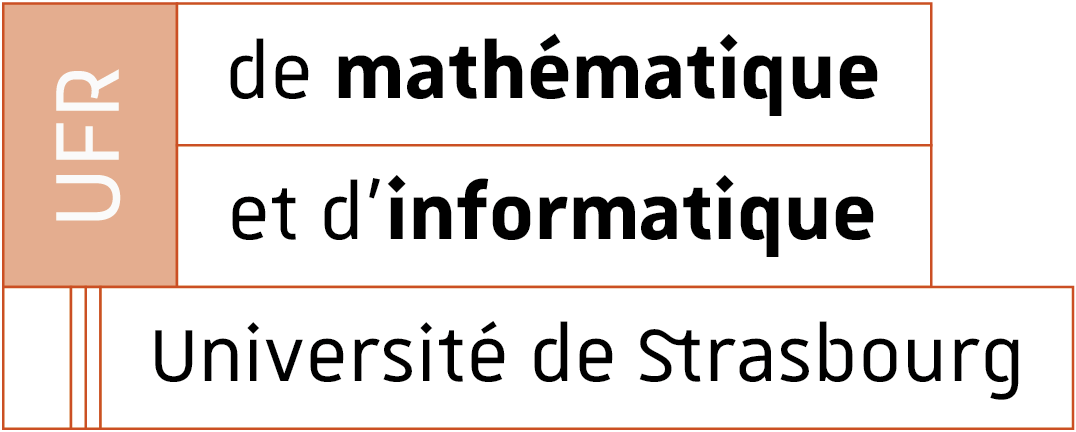
\includegraphics[width=0.5\textwidth]{images/logo_ufr.png}\par\vspace{1cm}
\vspace{1.5cm}
{\huge\bfseries ExaMA WP1 - Vegetation\par}
\vspace{2cm}
{\Large Giulio Carpi Lapi, Pierre-Antoine Senger\par}
\vfill
supervised by\par
Pierre Alliez and Vincent Chabannes

\vfill

% Bottom of the page
{\large Date: \today\par}
\end{titlepage}

\tableofcontents
\newpage

\section{Abstract}
Urban areas are complex ecosystems influenced by various factors, among which 
vegetation, especially trees, holds significant importance. Trees play a crucial 
role in shaping microclimates, reducing energy consumption, and enhancing overall 
livability\cite{TIR4sTREEt}. This project aims to integrate vegetation, specifically trees, into 3D 
geometric models of urban environments to improve the accuracy and realism of thermal 
and energy simulations. Utilizing data from open sources like \texttt{OpenStreetMap},
we identified tree positions and attributes and developped a library of 3D tree
models for integration into terrain meshes.

The project follows a roadmap with defined milestones to deliver versions
\texttt{V0}, \texttt{V1}, and \texttt{V2} by specified  deadlines.

\subsection{Main Objectives}

The primary objective is to enhance the accuracy of thermal and energy
simulations of a given area.

Specific objectives include:
\begin{itemize}
    \item Extracting tree data from \texttt{OpenStreetMap}
    \item Generating 3D tree models.
    \item Integrating tree models into terrain meshes.
    \item Simulating how trees influence energy consumption and microclimates.
    \item Optimizing computational efficiency
    \item Delivering versions \texttt{V0}, \texttt{V1}, and \texttt{V2} by specified deadlines
\end{itemize}

\section{Introduction}
Urban areas are intricate environments influenced by a multitude of factors, with 
vegetation, notably trees, playing a pivotal role in shaping their microclimates 
and energy dynamics. Trees provide shade and heat mitigation making them
indispensable elements in urban landscapes\cite{TIR4sTREEt,img:TreeShade}.

\begin{figure}[H]
    \centering
    \begin{minipage}{0.45\textwidth}
        \centering
        \includegraphics[width=\textwidth]{images/TreeShade.png}
        \captionsetup{font={scriptsize}}
        \caption{Tree providing shade to a buiding \cite{img:TreeShade}.}
    \end{minipage}\hfill
    \begin{minipage}{0.45\textwidth}
        \centering
        \includegraphics[width=\textwidth]{images/heat_street.png}
        \captionsetup{font={scriptsize}}
        \caption{Thermal image of a street depicting heat distribution \cite{img:street_thermography}.}
    \end{minipage}
\end{figure}

Computational modeling has advanced significantly, enabling the simulation of thermal 
and energy performance in urban environments. However, integrating vegetation into 
these models presents challenges due to the complexity of obtaining accurate tree data 
and representing their geometry efficiently\cite{AdTree}.

\newpage

\subsection{Challenges}
This project aims to address these challenges by developing a methodology for 
integrating trees into 3D urban models. Leveraging data from \texttt{OpenStreetMap},
the  project will identify tree positions and attributes, generate a library of 3D tree 
models, and integrate them into terrain meshes for comprehensive simulations while
ensuring computational efficiency.

\subsection{Structure of the Report}

The report will be structured as follows:

\begin{enumerate}
    \item \textbf{Abstract}: A concise summary of the project's objectives, methodologies, 
    and key findings.
    
    \item \textbf{Introduction}: An overview of the importance of vegetation in urban areas, 
    the challenges in integrating it into 3D models, and the objectives of the project.
    
    \item \textbf{Methodology}: Detailed explanation of the steps involved in data acquisition, 
    tree model generation, model integration and the running of thermal simulations.
    
    \item \textbf{Results}: Presentation of the outcomes and findings obtained from the 
    implemented methodology.
    
    \item \textbf{Conclusion}: Summary of the project's achievements, implications, and 
    potential future work.
    
    \item \textbf{References}: List of all the sources cited in the report.
\end{enumerate}

Each section will be elaborated upon in detail to provide a comprehensive understanding 
of the project's scope, approach, and outcomes.


\subsection{Data Formats and Structure}
Tree data will be sourced from \texttt{OpenStreetMap} and processed into formats suitable for 
integration into our models, such as \texttt{.off}, \texttt{.csv}, and \texttt{.json}.
We aim to ensure watertight triangulation consistent with the Finite Element Method
(FEM) for accurate simulations.  

The .off format\cite{off_format} is a simple format for 3D or 4D objects consisting of: (for 3D objects)
\begin{itemize}
    \item The keyword OFF
    \item The number of vertices, faces, and edges in order 
    \item A list of vertices: X, Y, Z coordinates
    \item A list of faces : number of vertices, vertex indices, in order (optionally, an RGB color)
\end{itemize}

\subsection{Software and Libraries}
To source our data, we'll utilize the \texttt{Overpass API} \cite{overpass} alongside
\texttt{curl} \cite{curl} to access and leverage information from \texttt{OpenStreetMap}.
For geometric modeling, we will utilize the \texttt{CGAL} \cite{cgal} library, known for its efficiency and 
reliability in geometric computation. Shading calculations will be performed using the 
\texttt{Feel++} \cite{feel++} library, which specializes in solving Partial Differential Equations (PDEs) 
essential for simulating light and shade on 3D objects.

\subsection{GitHub Repository}
We created a \texttt{GitHub} repository to manage the project and facilitate collaboration.
The repository contains the project's code, documentation, and resources. It will be
updated regularly to reflect the progress and changes made during the project's
development.

\subsection{Roadmap}
As of \texttt{V0} (March 2024) the roadmap we defined includes the following
milestones and issues:
\begin{figure}[H]
    \centering
    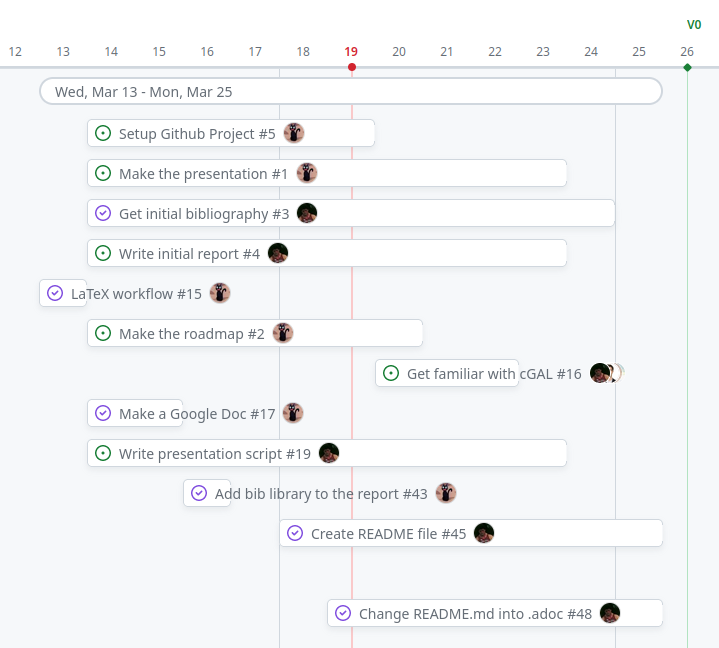
\includegraphics[width=1\textwidth]{images/roadmap_v0.png}
    \captionsetup{font={scriptsize}}
    \caption{Roadmap for V0}
\end{figure}

\begin{figure}[H]
    \centering
    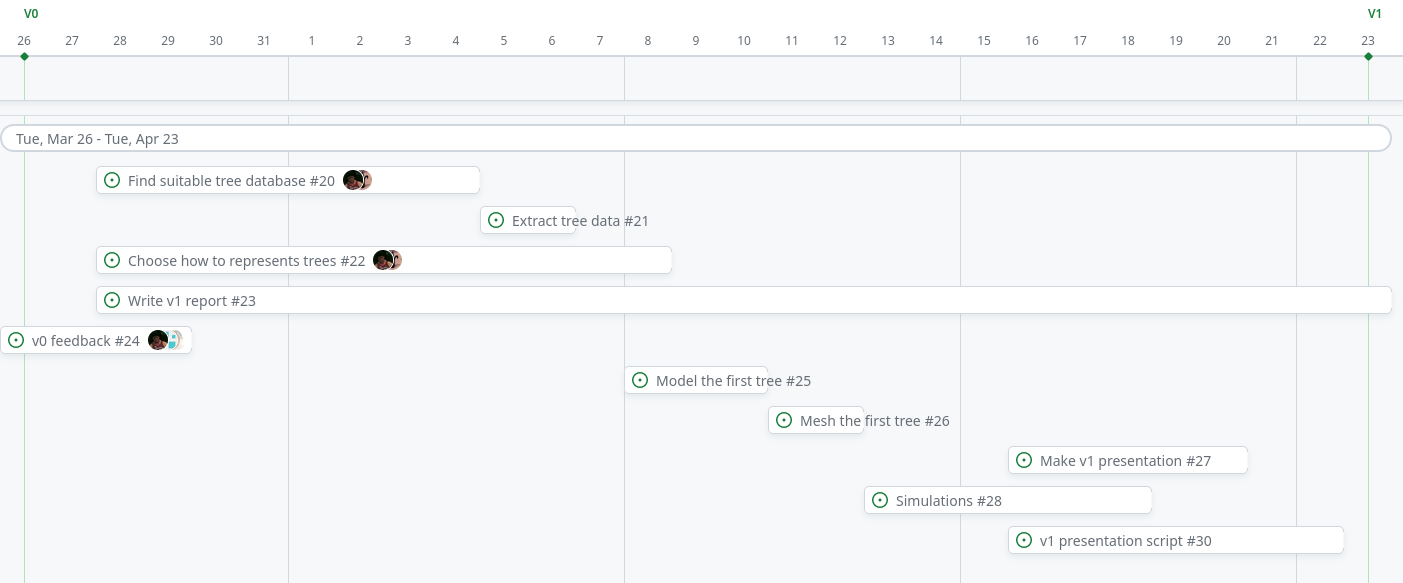
\includegraphics[width=1\textwidth]{images/roadmap_v1.png}
    \captionsetup{font={scriptsize}}
    \caption{Roadmap for V1}
\end{figure}

\begin{figure}[H]
    \centering
    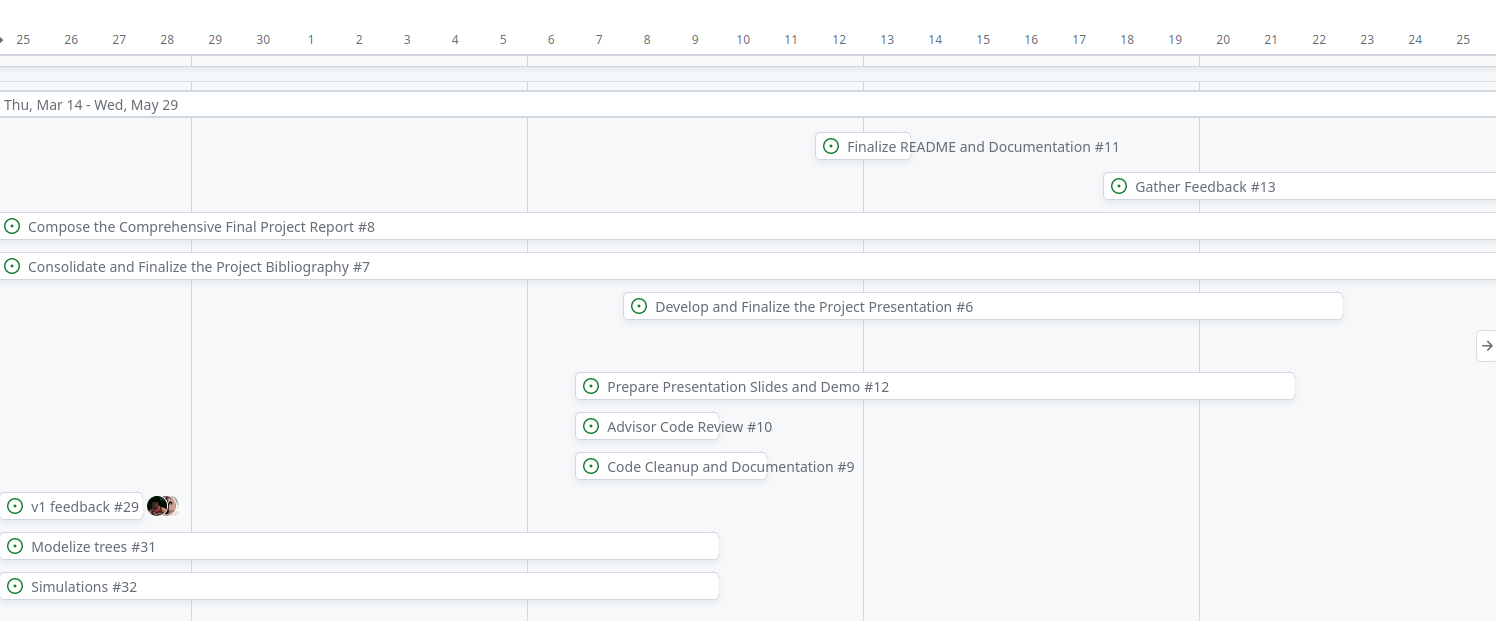
\includegraphics[width=1\textwidth]{images/roadmap_v2.png}
    \captionsetup{font={scriptsize}}
    \caption{Roadmap for V2}
\end{figure}

\newpage

\section{Methodology}

\subsection{Data Acquisition}
A \textit{config.json} file will be available for the user to specify the area of
interest. The file contains the latitude and longitude of two points, A and B,
which define a bounding box.

Here's an example of the \textit{config.json} file for the Strasbourg, France
city center:

\begin{lstlisting}[language=json,firstnumber=1]
{
    "A": {
        "latitude": 48.578702,
        "longitude": 7.739103
    },
    "B": {
        "latitude": 48.587756,
        "longitude": 7.756632
    }
}
\end{lstlisting}

We will then use the \texttt{Overpass API} to query \texttt{OpenStreetMap}
for all the available tree data within the specified bounding box.
The data will be stored in a \textit{.json} file.

\newpage
Here's an example of the result of the query for one tree:

\begin{lstlisting}[language=json,firstnumber=1]
{
    "type": "node",
    "id": 10161978695,
    "lat": 48.5872478,
    "lon": 7.7548520,
    "tags": {
        "circumference": "78.54",
        "diameter_crown": "5",
        "genus": "Tilia",
        "height": "10",
        "natural": "tree",
        "ref": "27466",
        "source": "data.strasbourg.eu - patrimoine_arbore",
        "source:date": "2022-01-02",
        "species": "Tilia euchlora x"
    }
}
\end{lstlisting}

We will especially use the \texttt{position} of the tree (latitude and longitude),
its \texttt{height}, the \texttt{diameter of its foliage}, and the \texttt{species}
to generate the 3D tree models.

\subsection{Tree Library}

\subsection{Tree Model Generation}
Using CGAL Alpha Wrapper \cite{cgal_alpha_wrapper}, 3D tree models will be generated based on the extracted data. Various 
Levels of Detail (LOD) will be considered to balance model complexity and computational 
efficiency depending on the application.

\subsection{Model Integration}
Generated tree models will be integrated into terrain meshes to create comprehensive 
3D urban models. Watertight triangulation consistent with FEM principles will be ensured 
for accurate simulations.

\subsection{Shading Calculations}
Using \texttt{Feel++} ray tracing, shading effects on buildings will be simulated to account for the presence 
of trees and their impact on urban microclimates. Execution time considerations will be 
addressed to optimize computational efficiency.

\newpage

\section{Results}


\newpage

\section{Conclusion}


\newpage

\section{References}
\bibliographystyle{unsrt}
\bibliography{references}

\end{document}
